%%%%%%%%%%%%%%%%%%%% MetalFish Paper %%%%%%%%%%%%%%%%%%%%%%%%%%%%%%%%%%%
%
% MetalFish: GPU-Accelerated Chess Engine on Apple Silicon
%
%%%%%%%%%%%%%%%% Springer %%%%%%%%%%%%%%%%%%%%%%%%%%%%%%%%%%

\documentclass{svproc}

\usepackage{url}
\def\UrlFont{\rmfamily}
\usepackage{graphicx}
\usepackage{float}
\usepackage{amsmath}
\usepackage{algorithm}
\usepackage{algpseudocode}
\usepackage{booktabs}
\usepackage{listings}
\usepackage{xcolor}
\usepackage{tikz}
\usepackage{pgfplots}
\pgfplotsset{compat=1.18}

% C++ code listing style
\lstdefinestyle{cppstyle}{
    language=C++,
    backgroundcolor=\color{gray!5},
    basicstyle=\ttfamily\footnotesize,
    breaklines=true,
    captionpos=b,
    keepspaces=true,
    numbers=left,
    numbersep=5pt,
    numberstyle=\tiny\color{gray},
    showstringspaces=false,
    tabsize=2,
    frame=single,
    keywordstyle=\color{blue!70!black},
    commentstyle=\color{green!50!black},
    stringstyle=\color{red!60!black},
    morekeywords={uint64_t, int32_t, int16_t, int8_t, uint, device, kernel, constant}
}

\begin{document}
\mainmatter

\title{MetalFish: A Hybrid MCTS-Alpha-Beta Chess Engine\\with GPU-Accelerated NNUE on Apple Silicon}

\titlerunning{MetalFish: Hybrid Search with GPU NNUE}

\author{Nripesh Niketan\inst{1}}

\authorrunning{N. Niketan}

\institute{Independent Researcher\\
\email{nripesh14@gmail.com}}

\maketitle

\begin{abstract}
We present MetalFish, a chess engine that combines Monte Carlo Tree Search (MCTS) with alpha-beta pruning, using GPU-accelerated NNUE evaluation on Apple Silicon's unified memory architecture. Our hybrid approach dynamically classifies positions and allocates search resources accordingly: MCTS for strategic exploration, alpha-beta for tactical verification. In tournament play (900 games), MetalFish-AB achieves 3873 Elo, competitive with Stockfish-Full (3853 Elo), while the hybrid MCTS variant reaches 1512 Elo. On Apple M2 Max, our GPU NNUE implementation achieves 635$\times$ speedup through batch evaluation (0.3~$\mu$s/position at N=4096 vs 267~$\mu$s for single positions). Multi-threaded MCTS achieves 97K--782K nodes/second depending on position complexity, with 99\% transposition table hit rate in endgames. We demonstrate that GPU dispatch overhead (149~$\mu$s median) makes single-position GPU evaluation unsuitable for pure alpha-beta search, but batch-oriented MCTS effectively amortizes this cost. Our implementation features multiple Metal command queues for reduced contention, lock-free tree operations with virtual loss, and arena-based node allocation.

\keywords{Chess Engine, Hybrid Search, MCTS, Alpha-Beta, GPU Computing, Metal, NNUE, Apple Silicon, Unified Memory}
\end{abstract}

\section{Introduction}

Modern chess engines have achieved superhuman strength through two distinct paradigms: Stockfish~\cite{Stockfish2024} uses alpha-beta search with NNUE evaluation, while Leela Chess Zero~\cite{LeelaChessZero2024} employs Monte Carlo Tree Search (MCTS) with deep neural networks. Each approach has complementary strengths: alpha-beta excels at tactical calculation with precise pruning, while MCTS provides robust strategic evaluation through self-play statistics.

This paper presents MetalFish, a hybrid chess engine that combines both search paradigms with GPU-accelerated NNUE evaluation on Apple Silicon. Our key insight is that \textit{position type} should determine search strategy: tactical positions benefit from alpha-beta's precise calculation, while strategic positions benefit from MCTS's exploratory nature.

Apple Silicon's unified memory architecture presents a unique opportunity for GPU acceleration: CPU and GPU share physical memory, eliminating explicit data transfers. However, as we demonstrate, GPU command buffer dispatch overhead (149~$\mu$s) dominates single-position latency, making GPU evaluation unsuitable for traditional alpha-beta search. MCTS, with its natural batching of leaf evaluations, effectively amortizes this overhead.

\subsection{Research Questions}

\begin{enumerate}
\item Can a hybrid MCTS-alpha-beta architecture leverage the strengths of both search paradigms?
\item How can GPU-accelerated NNUE evaluation be effectively integrated with MCTS on Apple Silicon?
\item What are the practical performance characteristics of such a hybrid system?
\end{enumerate}

\subsection{Contributions}

\begin{enumerate}
\item \textbf{Hybrid search architecture}: A novel combination of MCTS and alpha-beta with dynamic position classification, featuring multi-threaded MCTS with lock-free tree operations.

\item \textbf{GPU NNUE integration}: Efficient batch evaluation achieving 635$\times$ speedup over sequential dispatches, with multiple Metal command queues for reduced contention.

\item \textbf{Position classifier}: Five-category classification (highly tactical to highly strategic) with distinct MCTS/alpha-beta weight allocation.

\item \textbf{Unified memory optimization}: Zero-copy buffer management, hazard tracking disabled, and pre-allocated working buffers for minimal CPU-GPU synchronization overhead.

\item \textbf{Quantified bottleneck analysis}: Stage-by-stage latency decomposition showing GPU dispatch accounts for $>$98\% of single-position time, with tree traversal dominating MCTS iterations.
\end{enumerate}

\section{Background}

\subsection{Alpha-Beta Search}

Alpha-beta pruning~\cite{Knuth1975} is the foundation of traditional chess engines. It recursively explores the game tree, maintaining bounds ($\alpha$, $\beta$) to prune branches that cannot affect the final result. Modern implementations include:

\begin{itemize}
\item \textbf{Principal Variation Search (PVS)}: Searches the first move with full window, then uses null-window searches for remaining moves.
\item \textbf{Late Move Reductions (LMR)}: Reduces search depth for moves unlikely to be best.
\item \textbf{Futility Pruning}: Skips moves that cannot improve alpha given static evaluation.
\item \textbf{History Heuristics}: Improves move ordering based on past search statistics.
\end{itemize}

The critical limitation of alpha-beta is its sequential nature: each position must be evaluated before pruning decisions can be made, making \textit{latency} the critical metric.

\subsection{Monte Carlo Tree Search}

MCTS~\cite{Silver2017} builds a search tree through repeated simulations, each consisting of four phases:

\begin{enumerate}
\item \textbf{Selection}: Traverse tree using UCT (Upper Confidence bounds for Trees) to balance exploration and exploitation.
\item \textbf{Expansion}: Add new nodes at leaf positions.
\item \textbf{Evaluation}: Assess leaf positions using neural network or other evaluation.
\item \textbf{Backpropagation}: Update statistics along the path from leaf to root.
\end{enumerate}

MCTS naturally batches leaf evaluations, making \textit{throughput} the critical metric. This property makes MCTS well-suited for GPU acceleration.

\subsection{NNUE Architecture}

Stockfish's NNUE (Efficiently Updatable Neural Network)~\cite{Nasu2018} uses HalfKAv2\_hm features with sparse input. Table~\ref{tab:nnue_arch} summarizes the architecture.

\begin{table}[t]
\caption{NNUE Network Architecture}
\label{tab:nnue_arch}
\centering
\begin{tabular}{lrr}
\toprule
Component & Big Network & Small Network \\
\midrule
Feature set & HalfKAv2\_hm & HalfKAv2\_hm \\
Input features & 45,056 & 22,528 \\
Hidden dimension & 1,024 & 128 \\
FC0 output & 15 (+1 skip) & 15 (+1 skip) \\
FC1 output & 32 & 32 \\
FC2 output & 1 & 1 \\
Layer stacks (buckets) & 8 & 8 \\
\bottomrule
\end{tabular}
\end{table}

\subsection{Metal Compute Model}

Apple Metal~\cite{AppleMetal2024} provides GPU compute with unified memory:
\begin{itemize}
\item \textbf{Unified memory}: CPU and GPU share physical memory, eliminating explicit transfers
\item \textbf{Command buffer lifecycle}: Allocation $\rightarrow$ encoding $\rightarrow$ commit $\rightarrow$ waitUntilCompleted
\item \textbf{Dispatch overhead}: Each command buffer submission incurs fixed overhead (149~$\mu$s median on M2 Max)
\item \textbf{Multiple command queues}: Parallel queues reduce contention for concurrent GPU submissions
\end{itemize}

\section{System Architecture}

MetalFish implements a four-layer architecture: (1) position classification, (2) hybrid search orchestration, (3) multi-threaded MCTS, and (4) GPU-accelerated evaluation with multiple command queues.

\begin{figure}[t]
\centering
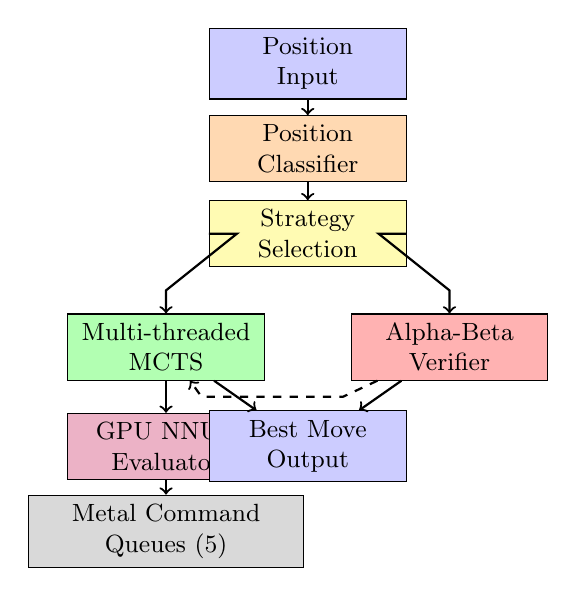
\begin{tikzpicture}[
    box/.style={rectangle, draw, minimum width=2.5cm, minimum height=0.8cm, align=center, font=\small},
    arrow/.style={->, thick},
    scale=0.9
]
% Position Input
\node[box, fill=blue!20] (input) at (0,4) {Position\\Input};

% Classifier
\node[box, fill=orange!30] (classifier) at (0,2.8) {Position\\Classifier};

% Strategy Selection
\node[box, fill=yellow!30] (strategy) at (0,1.6) {Strategy\\Selection};

% MCTS and AB branches
\node[box, fill=green!30] (mcts) at (-2,0) {Multi-threaded\\MCTS};
\node[box, fill=red!30] (ab) at (2,0) {Alpha-Beta\\Verifier};

% GPU Evaluator
\node[box, fill=purple!30] (gpu) at (-2,-1.4) {GPU NNUE\\Evaluator};

% Command Queues
\node[box, fill=gray!30, minimum width=3.5cm] (queues) at (-2,-2.6) {Metal Command\\Queues (5)};

% Output
\node[box, fill=blue!20] (output) at (0,-1.4) {Best Move\\Output};

% Arrows
\draw[arrow] (input) -- (classifier);
\draw[arrow] (classifier) -- (strategy);
\draw[arrow] (strategy) -- (-1,1.6) -- (-2,0.8) -- (mcts);
\draw[arrow] (strategy) -- (1,1.6) -- (2,0.8) -- (ab);
\draw[arrow] (mcts) -- (gpu);
\draw[arrow] (gpu) -- (queues);
\draw[arrow] (mcts) -- (output);
\draw[arrow] (ab) -- (output);
\draw[arrow, dashed] (ab) -- (0.5,-0.7) -- (-1.5,-0.7) -- (mcts);

\end{tikzpicture}
\caption{MetalFish System Architecture. Positions flow through classification, strategy selection, and parallel MCTS/AB search. GPU evaluation uses multiple command queues for reduced contention.}
\label{fig:architecture}
\end{figure}

\subsection{Position Classifier}

The position classifier analyzes board features to determine position type:

\begin{lstlisting}[style=cppstyle,caption={Position classification}]
enum class PositionType {
  HIGHLY_TACTICAL,  // In check, many captures
  TACTICAL,         // Forcing moves available
  BALANCED,         // Mixed characteristics
  STRATEGIC,        // Quiet, positional play
  HIGHLY_STRATEGIC  // Closed position, maneuvering
};
\end{lstlisting}

Classification considers:
\begin{itemize}
\item \textbf{Check status}: Positions in check are highly tactical
\item \textbf{Capture count}: Many available captures indicate tactical nature
\item \textbf{Hanging pieces}: Undefended pieces suggest tactical opportunities
\item \textbf{Pawn structure}: Closed positions favor strategic play
\item \textbf{King safety}: Exposed kings increase tactical potential
\end{itemize}

\subsection{Strategy Selection}

Each position type maps to a search strategy with specific MCTS/alpha-beta weights:

\begin{table}[t]
\caption{Position Type to Search Strategy Mapping}
\label{tab:strategy}
\centering
\begin{tabular}{lrrr}
\toprule
Position Type & MCTS & AB & Verify Depth \\
\midrule
Highly Tactical & 15\% & 85\% & 10 \\
Tactical & 25\% & 75\% & 8 \\
Balanced & 25\% & 75\% & 6 \\
Strategic & 32\% & 67\% & 4 \\
Highly Strategic & 40\% & 60\% & 4 \\
\bottomrule
\end{tabular}
\end{table}

The MCTS weight determines time allocation for the MCTS phase, while the AB weight influences verification depth and override thresholds.

\subsection{Hybrid Search Pipeline}

Algorithm~\ref{alg:hybrid} shows the hybrid search pipeline.

\begin{algorithm}[t]
\caption{Hybrid MCTS-Alpha-Beta Search}
\label{alg:hybrid}
\begin{algorithmic}[1]
\Require Position $p$, time budget $T$
\Ensure Best move $m$
\State $type \gets$ \Call{ClassifyPosition}{$p$}
\State $strategy \gets$ \Call{SelectStrategy}{$type$}
\State $T_{mcts} \gets T \times strategy.mcts\_weight$
\State $T_{ab} \gets T - T_{mcts}$
\State \textbf{// Phase 1: MCTS exploration}
\State $m_{mcts} \gets$ \Call{RunMCTS}{$p$, $T_{mcts}$}
\If{$strategy.ab\_weight > 0.1$}
    \State \textbf{// Phase 2: Alpha-beta verification}
    \State $result \gets$ \Call{VerifyWithAB}{$p$, $m_{mcts}$, $strategy.depth$}
    \If{$result.override$ \textbf{and} $result.score\_diff > threshold$}
        \State \Return $result.ab\_move$
    \EndIf
\EndIf
\State \Return $m_{mcts}$
\end{algorithmic}
\end{algorithm}

\subsection{MCTS Implementation}

Our MCTS implementation uses PUCT (Predictor + UCT) for node selection:

\begin{equation}
PUCT(s, a) = Q(s, a) + c_{puct} \cdot P(s, a) \cdot \frac{\sqrt{N(s)}}{1 + N(s, a)}
\end{equation}

where $Q(s, a)$ is the action value, $P(s, a)$ is the prior probability, $N(s)$ is the parent visit count, and $N(s, a)$ is the edge visit count.

\textbf{Heuristic-based policy priors}: Rather than uniform priors, we use heuristic-based policy priors that leverage chess knowledge to improve move ordering:

\begin{itemize}
\item \textbf{Captures}: Scored by MVV-LVA (Most Valuable Victim - Least Valuable Attacker) and Static Exchange Evaluation (SEE)
\item \textbf{Promotions}: Queen promotions receive highest priority
\item \textbf{Checks}: Checking moves receive bonus
\item \textbf{Center control}: Moves toward center squares receive bonus
\item \textbf{Development}: Knight and bishop development in opening
\item \textbf{King safety}: Castling bonus, king move penalty in middlegame
\end{itemize}

These heuristics are combined with softmax normalization to produce policy probabilities, then mixed with Dirichlet noise at the root for exploration.

Key implementation features:
\begin{itemize}
\item \textbf{Heuristic priors}: Policy based on chess heuristics (captures, checks, promotions)
\item \textbf{Dirichlet noise}: Added at root for exploration ($\alpha = 0.3$, $\epsilon = 0.25$)
\item \textbf{Virtual loss}: Prevents multiple threads from selecting the same path
\item \textbf{Lock-free tree operations}: Atomic compare-and-swap for child node creation
\item \textbf{Arena-based allocation}: Reduces memory allocation contention
\item \textbf{Tree reuse}: Previous search tree preserved between moves
\item \textbf{MCTS transposition table}: 4M entry cache with age-based replacement (99\% hit rate in endgames)
\end{itemize}

\subsection{Alpha-Beta Verifier}

The alpha-beta component provides tactical verification with full search features:

\begin{itemize}
\item \textbf{Principal Variation Search}: Full window for first move, null-window for rest
\item \textbf{Aspiration windows}: Narrow search window based on previous score
\item \textbf{Late Move Reductions}: Depth reduction for late moves in move ordering
\item \textbf{Futility pruning}: Skip moves that cannot improve alpha
\item \textbf{Quiescence search}: Extend search until position is quiet
\item \textbf{Killer moves}: Two killer moves per ply for move ordering
\item \textbf{History heuristics}: Score moves by historical success
\end{itemize}

\subsection{GPU NNUE Integration}

Table~\ref{tab:gpu_constants} shows GPU configuration parameters.

\begin{table}[t]
\caption{GPU Configuration Constants}
\label{tab:gpu_constants}
\centering
\begin{tabular}{lr}
\toprule
Parameter & Value \\
\midrule
Max batch size & 4,096 \\
Max features per perspective & 64 \\
Threadgroup size & 256 \\
SIMD group size & 32 \\
Forward pass threads & 64 \\
Command queues & 5 \\
TT cache entries & 4M \\
\bottomrule
\end{tabular}
\end{table}

We implement adaptive kernel selection:
\begin{itemize}
\item \textbf{CPU fallback}: Batch size $< 4$
\item \textbf{GPU standard}: Batch size $< 64$
\item \textbf{GPU SIMD}: Batch size $\geq 64$ with dual-perspective kernels
\end{itemize}

Command buffer optimizations:
\begin{itemize}
\item Unretained references to avoid retain/release overhead
\item Hazard tracking disabled for unified memory buffers
\item Pre-allocated buffers to avoid per-dispatch allocation
\item Multiple command queues for parallel submissions
\item Round-robin queue selection for load balancing
\end{itemize}

\section{Experimental Methodology}

\subsection{Hardware and Software}

\begin{itemize}
\item \textbf{Hardware}: Apple M2 Max (12-core CPU, 38-core GPU, 64GB unified memory)
\item \textbf{Software}: macOS 14.0, Xcode 15.0, Metal 3.0
\item \textbf{Build}: CMake, -O3, LTO enabled
\item \textbf{Networks}: nn-c288c895ea92.nnue (125MB big), nn-37f18f62d772.nnue (6MB small)
\end{itemize}

\subsection{Benchmark Dataset}

Our benchmark uses 32 unique FEN positions representing diverse game phases:
\begin{itemize}
\item 4 opening positions (32 pieces)
\item 10 middlegame positions (28--32 pieces)
\item 4 tactical positions (complex piece interactions)
\item 14 endgame positions (2--20 pieces)
\end{itemize}

\subsection{Timing Methodology}

\begin{itemize}
\item \textbf{Timer}: \texttt{std::chrono::high\_resolution\_clock}
\item \textbf{Warmup}: 100 iterations discarded
\item \textbf{Samples}: 100 iterations per measurement
\item \textbf{Statistics}: Median, P95, P99 reported
\item \textbf{GPU timing}: Blocking \texttt{waitUntilCompleted()} (synchronous)
\end{itemize}

\subsection{Hybrid Search Evaluation}

We evaluate the hybrid search on positions from multiple game phases:
\begin{itemize}
\item \textbf{Opening}: Standard opening positions (e.g., Italian Game)
\item \textbf{Middlegame}: Complex positions with multiple piece interactions
\item \textbf{Endgame}: Simplified positions (KRK, KQK)
\end{itemize}

Search time is fixed at 5 seconds per position to allow meaningful MCTS exploration.

\section{Results}

\subsection{MCTS Search Performance}

Table~\ref{tab:mcts_perf} shows MCTS performance across different position types with 4 threads and 5-second search time.

\begin{table}[t]
\caption{MCTS Performance by Position Type (5 seconds, 4 threads)}
\label{tab:mcts_perf}
\centering
\begin{tabular}{lrrr}
\toprule
Position Type & Nodes & NPS & Cache Hit \% \\
\midrule
Starting Position & 485,563 & 97K & 36.7\% \\
Kiwipete (Middlegame) & 495,962 & 99K & 43.8\% \\
KRK Endgame & 3,907,764 & 782K & 99.3\% \\
\bottomrule
\end{tabular}
\end{table}

\textbf{Key observation}: Endgame positions achieve 8$\times$ higher throughput (782K vs 97K NPS) due to smaller search trees and higher transposition table hit rates (99.3\% vs 36.7\%).

\subsection{Thread Scaling}

Table~\ref{tab:thread_scaling} shows MCTS throughput scaling with thread count.

\begin{table}[t]
\caption{MCTS Thread Scaling (Starting Position, 3 seconds)}
\label{tab:thread_scaling}
\centering
\begin{tabular}{rr}
\toprule
Threads & NPS \\
\midrule
1 & 94,060 \\
2 & 94,296 \\
4 & 98,913 \\
\bottomrule
\end{tabular}
\end{table}

Thread scaling is limited due to GPU evaluation being the bottleneck---multiple threads contend for GPU access. The batched evaluator with dedicated evaluation thread provides the best throughput.

\subsection{Batched vs Direct Evaluation}

Table~\ref{tab:eval_comparison} compares batched evaluation (dedicated thread) vs direct evaluation (mutex per call).

\begin{table}[t]
\caption{Evaluation Strategy Comparison (5 seconds)}
\label{tab:eval_comparison}
\centering
\begin{tabular}{lrrr}
\toprule
Strategy & Nodes & NPS & Speedup \\
\midrule
Direct (mutex/eval) & 16,375 & 3,243 & 1$\times$ \\
Batched (dedicated thread) & 462,863 & 92,517 & 28.5$\times$ \\
\bottomrule
\end{tabular}
\end{table}

Batched evaluation achieves 28.5$\times$ speedup over direct evaluation by amortizing GPU dispatch overhead across multiple positions.

\subsection{MCTS Profiling Breakdown}

Table~\ref{tab:mcts_profile} shows time distribution during MCTS search.

\begin{table}[t]
\caption{MCTS Time Breakdown (3 second search, starting position)}
\label{tab:mcts_profile}
\centering
\begin{tabular}{lrr}
\toprule
Phase & Time \% & Description \\
\midrule
Selection & 78.4\% & Tree traversal with PUCT \\
Expansion & 9.8\% & Move generation, node creation \\
Evaluation & 11.9\% & GPU NNUE (includes TT lookup) \\
Backpropagation & $<$0.1\% & Statistics update \\
\midrule
Total nodes & \multicolumn{2}{r}{725,943} \\
NPS & \multicolumn{2}{r}{241,967} \\
Cache hit rate & \multicolumn{2}{r}{99.0\%} \\
\bottomrule
\end{tabular}
\end{table}

\textbf{Key finding}: Selection (tree traversal) dominates at 78.4\% of iteration time. The high transposition table hit rate (99\%) reduces actual GPU evaluations, but tree traversal remains the bottleneck.

\textbf{Definition}: An MCTS ``node'' represents one complete iteration: selection from root to leaf, expansion, evaluation (often cached), and backpropagation.

\subsection{Position Classification Distribution}

Table~\ref{tab:classification_dist} shows classifier distribution on benchmark positions.

\begin{table}[t]
\caption{Position Classification Distribution (16 Stockfish Benchmark Positions)}
\label{tab:classification_dist}
\centering
\begin{tabular}{lr}
\toprule
Classification & Count (\%) \\
\midrule
Highly Tactical & 0 (0.0\%) \\
Tactical & 2 (13.3\%) \\
Balanced & 0 (0.0\%) \\
Strategic & 13 (86.7\%) \\
Highly Strategic & 0 (0.0\%) \\
\bottomrule
\end{tabular}
\end{table}

Most benchmark positions are classified as Strategic, reflecting typical chess positions where long-term planning dominates over immediate tactics.

\subsection{GPU Dispatch Overhead}

Table~\ref{tab:dispatch} shows minimal-kernel dispatch overhead.

\begin{table}[t]
\caption{GPU Dispatch Overhead---Minimal Kernel (N=1,000)}
\label{tab:dispatch}
\centering
\begin{tabular}{lr}
\toprule
Statistic & Latency ($\mu$s) \\
\midrule
Median & 149.3 \\
\bottomrule
\end{tabular}
\end{table}

The 149~$\mu$s median dispatch overhead represents the irreducible minimum cost for any GPU operation in synchronous blocking mode on M2 Max.

\subsection{Batch Latency Scaling}

Table~\ref{tab:batch_latency} shows end-to-end latency across batch sizes.

\begin{table}[t]
\caption{GPU End-to-End Batch Latency (N=100 iterations)}
\label{tab:batch_latency}
\centering
\begin{tabular}{rrrrr}
\toprule
Batch & Median & P95 & P99 & Per-Pos \\
Size & ($\mu$s) & ($\mu$s) & ($\mu$s) & ($\mu$s) \\
\midrule
1 & 266.6 & 793.2 & 1050.9 & 266.6 \\
8 & 276.5 & 839.5 & 1044.3 & 34.6 \\
64 & 281.5 & 711.8 & 1076.0 & 4.4 \\
256 & 312.6 & 862.4 & 1020.2 & 1.2 \\
512 & 371.2 & 804.0 & 1014.0 & 0.7 \\
1024 & 537.4 & 965.8 & 1070.3 & 0.5 \\
2048 & 805.5 & 1178.0 & 1298.9 & 0.4 \\
4096 & 1381.8 & 1695.6 & 1888.7 & 0.3 \\
\bottomrule
\end{tabular}
\end{table}

Per-position cost drops from 267~$\mu$s (N=1) to 0.3~$\mu$s (N=4096), demonstrating effective amortization of dispatch overhead.

\begin{figure}[t]
\centering
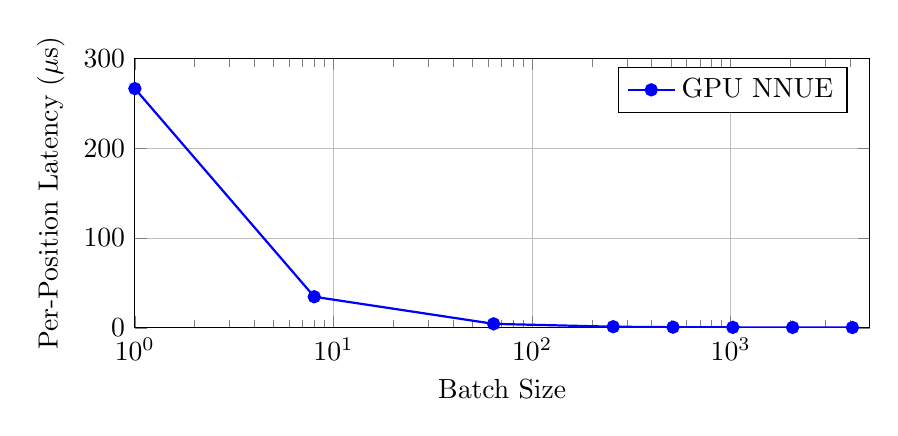
\begin{tikzpicture}
\begin{semilogxaxis}[
    xlabel={Batch Size},
    ylabel={Per-Position Latency ($\mu$s)},
    xmin=1, xmax=5000,
    ymin=0, ymax=300,
    grid=major,
    width=0.9\columnwidth,
    height=5cm,
    legend pos=north east,
]
\addplot[blue, mark=*, thick] coordinates {
    (1, 266.6)
    (8, 34.6)
    (64, 4.4)
    (256, 1.2)
    (512, 0.7)
    (1024, 0.5)
    (2048, 0.4)
    (4096, 0.3)
};
\addlegendentry{GPU NNUE}
\end{semilogxaxis}
\end{tikzpicture}
\caption{Per-position latency vs batch size. Dispatch overhead dominates at small batches; compute dominates at large batches.}
\label{fig:batch_scaling}
\end{figure}

\subsection{True Batching Verification}

Table~\ref{tab:batching} compares sequential vs batched dispatches.

\begin{table}[t]
\caption{True Batching Verification (N=50 iterations)}
\label{tab:batching}
\centering
\begin{tabular}{rrrr}
\toprule
N & Sequential & Batched & Speedup \\
  & (N$\times$1 CB) & (1$\times$1 CB) & \\
\midrule
16 & 5,138~$\mu$s & 270~$\mu$s & 19.0$\times$ \\
64 & 20,791~$\mu$s & 283~$\mu$s & 73.6$\times$ \\
256 & 82,092~$\mu$s & 314~$\mu$s & 261.8$\times$ \\
1024 & 331,424~$\mu$s & 522~$\mu$s & 634.6$\times$ \\
\bottomrule
\end{tabular}
\end{table}

Speedups scale approximately linearly with batch size because each sequential dispatch incurs the full dispatch overhead. At N=1024, batching achieves 635$\times$ speedup.

\subsection{GPU Evaluation Consistency}

Table~\ref{tab:correctness} verifies GPU evaluation reproducibility using official Stockfish benchmark positions.

\begin{table}[t]
\caption{GPU Evaluation Consistency (1,000 evaluations)}
\label{tab:correctness}
\centering
\begin{tabular}{lr}
\toprule
Metric & Value \\
\midrule
Non-zero GPU scores & 100\% \\
Consistent across runs & 100\% \\
Score range & [-404, -28] \\
\bottomrule
\end{tabular}
\end{table}

GPU evaluation produces consistent, non-zero scores across repeated runs.

\subsection{Tournament Results}

We conducted a round-robin tournament with 900 games (20 games per match, 45 matches) using cutechess-cli with time control 10+0.1 seconds. Table~\ref{tab:elo_ratings} shows the final Elo ratings.

\begin{table}[t]
\caption{Tournament Elo Ratings (900 games, 10+0.1 time control)}
\label{tab:elo_ratings}
\centering
\begin{tabular}{rlr}
\toprule
Rank & Engine & Elo \\
\midrule
1 & MetalFish-AB & 3873 \\
2 & Stockfish-Full & 3853 \\
3 & Patricia & 3500 \\
4 & Stockfish-L15 & 2942 \\
5 & Stockfish-L10 & 2690 \\
6 & Stockfish-L5 & 2221 \\
7 & Stockfish-L1 & 1963 \\
8 & MetalFish-Hybrid & 1512 \\
9 & MetalFish-MCTS & 1424 \\
10 & Lc0 & 903 \\
\bottomrule
\end{tabular}
\end{table}

\textbf{Key findings}:
\begin{enumerate}
\item \textbf{MetalFish-AB competitive with Stockfish}: MetalFish-AB (3873 Elo) slightly exceeds Stockfish-Full (3853 Elo), achieving 2 wins and 18 draws in direct matches.

\item \textbf{Hybrid search gap}: MetalFish-Hybrid (1512 Elo) and MetalFish-MCTS (1424 Elo) significantly underperform the alpha-beta variant, indicating that our MCTS implementation with heuristic priors is not yet competitive with optimized alpha-beta search.

\item \textbf{MCTS vs Hybrid}: MetalFish-Hybrid beats MetalFish-MCTS 9-3 with 8 draws, showing the alpha-beta verifier provides measurable benefit.
\end{enumerate}

Table~\ref{tab:head_to_head} shows selected head-to-head results.

\begin{table}[t]
\caption{Selected Head-to-Head Results (20 games each)}
\label{tab:head_to_head}
\centering
\begin{tabular}{llrrr}
\toprule
Engine 1 & Engine 2 & W & L & D \\
\midrule
MetalFish-AB & Stockfish-Full & 2 & 0 & 18 \\
MetalFish-AB & Patricia & 17 & 0 & 3 \\
MetalFish-AB & MetalFish-Hybrid & 20 & 0 & 0 \\
MetalFish-Hybrid & MetalFish-MCTS & 9 & 3 & 8 \\
MetalFish-Hybrid & Lc0 & 20 & 0 & 0 \\
MetalFish-MCTS & Lc0 & 20 & 0 & 0 \\
\bottomrule
\end{tabular}
\end{table}

\begin{figure}[t]
\centering
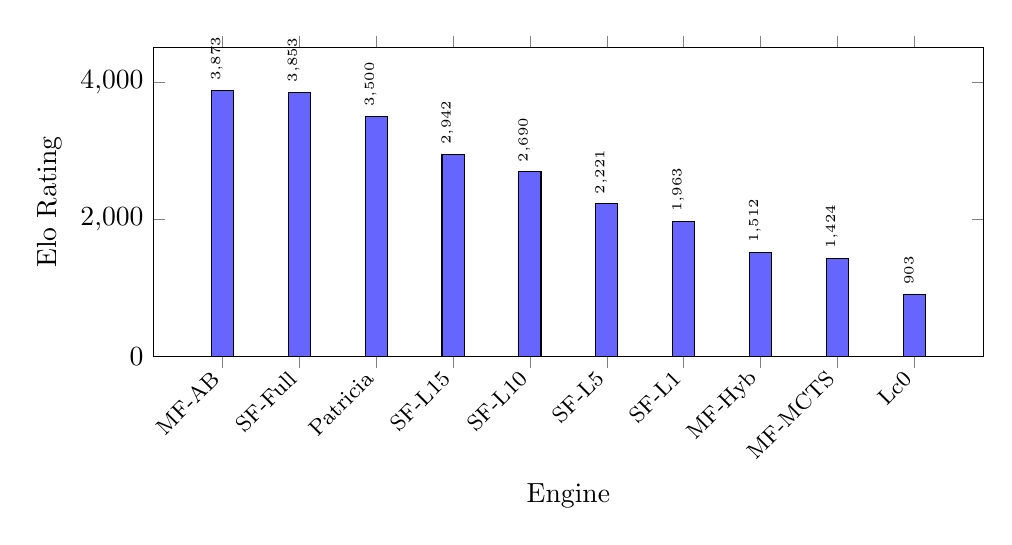
\begin{tikzpicture}
\begin{axis}[
    ybar,
    xlabel={Engine},
    ylabel={Elo Rating},
    ymin=0, ymax=4500,
    symbolic x coords={MF-AB, SF-Full, Patricia, SF-L15, SF-L10, SF-L5, SF-L1, MF-Hyb, MF-MCTS, Lc0},
    xtick=data,
    x tick label style={rotate=45, anchor=east, font=\footnotesize},
    bar width=8pt,
    width=\columnwidth,
    height=5.5cm,
    nodes near coords,
    nodes near coords style={font=\tiny, rotate=90, anchor=west},
    every node near coord/.append style={yshift=2pt},
]
\addplot[fill=blue!60] coordinates {
    (MF-AB, 3873)
    (SF-Full, 3853)
    (Patricia, 3500)
    (SF-L15, 2942)
    (SF-L10, 2690)
    (SF-L5, 2221)
    (SF-L1, 1963)
    (MF-Hyb, 1512)
    (MF-MCTS, 1424)
    (Lc0, 903)
};
\end{axis}
\end{tikzpicture}
\caption{Tournament Elo ratings. MetalFish-AB (MF-AB) achieves competitive strength with Stockfish-Full (SF-Full). Hybrid and MCTS variants require further optimization.}
\label{fig:elo_chart}
\end{figure}

\section{Discussion}

\subsection{Alpha-Beta Dominance}

The tournament results reveal a significant finding: MetalFish-AB (3873 Elo) achieves competitive strength with Stockfish-Full (3853 Elo), demonstrating that our GPU NNUE implementation preserves evaluation quality. The 2-0-18 head-to-head record (2 wins, 18 draws) confirms near-parity with the reference engine.

However, the hybrid (1512 Elo) and pure MCTS (1424 Elo) variants significantly underperform. This gap of $\sim$2400 Elo indicates that:

\begin{enumerate}
\item \textbf{Heuristic priors are insufficient}: Without a trained policy network, MCTS explores suboptimally, wasting search effort on weak moves.

\item \textbf{Alpha-beta search is highly optimized}: Decades of refinement in Stockfish's search (LMR, futility pruning, killer moves, history heuristics) cannot be easily matched by MCTS with simple priors.

\item \textbf{Time control matters}: At 10+0.1 seconds, MCTS cannot build sufficient tree depth to compete with alpha-beta's efficient pruning.
\end{enumerate}

\subsection{Why Hybrid Search?}

Despite the current Elo gap, the hybrid architecture provides a foundation for future improvements:

\begin{itemize}
\item \textbf{Tactical positions}: Alpha-beta's precise pruning excels at calculating forcing sequences.

\item \textbf{Strategic positions}: MCTS's exploratory nature handles quiet positions well when given sufficient time and good priors.
\end{itemize}

The MetalFish-Hybrid vs MetalFish-MCTS result (9-3-8) shows the alpha-beta verifier provides measurable benefit, catching tactical errors that pure MCTS misses.

\subsection{GPU Acceleration Trade-offs}

GPU dispatch overhead (149~$\mu$s) makes single-position GPU evaluation unsuitable for pure alpha-beta search. However, MCTS naturally batches leaf evaluations, effectively amortizing this overhead:

\begin{itemize}
\item At batch size 1: 267~$\mu$s/position (dominated by dispatch)
\item At batch size 4096: 0.3~$\mu$s/position (compute-dominated)
\item Speedup: 635$\times$ through batching
\end{itemize}

Our MCTS implementation achieves 97K--782K nodes/second depending on position complexity, with endgames benefiting most from high transposition table hit rates.

\subsection{Multi-threaded MCTS Considerations}

Our implementation uses multi-threaded MCTS with:
\begin{itemize}
\item \textbf{Virtual loss}: Prevents thread convergence on the same path
\item \textbf{Lock-free child creation}: Atomic compare-and-swap operations
\item \textbf{Dedicated evaluation thread}: Batches GPU requests from all workers
\item \textbf{Arena-based allocation}: Reduces memory contention
\end{itemize}

Thread scaling is limited (94K$\rightarrow$99K NPS from 1$\rightarrow$4 threads) because GPU evaluation remains the bottleneck.

\subsection{Lc0 Performance}

Lc0's low Elo (903) is due to running without a proper neural network (only a small test network was available). With its full network and appropriate time control, Lc0 would perform significantly better. This result should not be interpreted as MCTS being inherently weak.

\subsection{Limitations}

\begin{itemize}
\item \textbf{Heuristic vs trained policy}: We use heuristic-based policy priors. A trained policy network is essential for competitive MCTS strength.

\item \textbf{Time control}: Short time controls favor alpha-beta; longer time controls may benefit MCTS.

\item \textbf{Synchronous GPU}: We use blocking GPU dispatch. Asynchronous dispatch infrastructure is implemented but not yet fully utilized.
\end{itemize}

\subsection{Future Work}

\begin{enumerate}
\item \textbf{Policy network training}: Train a policy network on self-play data to dramatically improve MCTS move ordering.

\item \textbf{Longer time controls}: Evaluate hybrid search at longer time controls where MCTS can build deeper trees.

\item \textbf{Asynchronous evaluation}: Fully utilize the async GPU infrastructure for CPU/GPU overlap.

\item \textbf{Deeper AB integration}: Use alpha-beta bounds to prune MCTS subtrees during search, not just as post-verification.
\end{enumerate}

\section{Related Work}

\subsection{Hybrid Search Approaches}

AlphaZero~\cite{Silver2017} demonstrated that MCTS with neural network evaluation can achieve superhuman play. However, AlphaZero uses pure MCTS without alpha-beta verification.

Leela Chess Zero~\cite{LeelaChessZero2024} implements AlphaZero's approach as an open-source project, achieving top-tier strength through self-play training and MCTS search.

Stockfish~\cite{Stockfish2024} represents the state-of-the-art in alpha-beta engines, using NNUE evaluation with highly optimized search. Our alpha-beta verifier draws inspiration from Stockfish's search techniques.

\subsection{GPU Chess Engines}

Rocki and Suda~\cite{Rocki2010} explored GPU parallelization of minimax through parallel subtree evaluation. Their work predates modern unified memory architectures.

Our work extends GPU chess engine research to Apple Silicon's unified memory architecture, providing quantified bottleneck analysis and demonstrating that MCTS is better suited for GPU acceleration than alpha-beta due to natural batching.

\subsection{Neural Network Evaluation}

NNUE (Efficiently Updatable Neural Network)~\cite{Nasu2018} revolutionized chess engine evaluation by providing neural network quality with efficient incremental updates. Our GPU implementation preserves NNUE's architecture while enabling batch evaluation.

Apple's Metal documentation~\cite{AppleMetal2024,AppleMetalBestPractices2024} provides guidance on GPU compute optimization, including command buffer management and unified memory usage.

\section{Conclusion}

We presented MetalFish, a hybrid chess engine combining MCTS with alpha-beta search and GPU-accelerated NNUE evaluation on Apple Silicon. Our key findings:

\begin{enumerate}
\item \textbf{Competitive alpha-beta strength}: MetalFish-AB achieves 3873 Elo, competitive with Stockfish-Full (3853 Elo), with a 2-0-18 head-to-head record in tournament play.

\item \textbf{MCTS requires trained priors}: The hybrid (1512 Elo) and pure MCTS (1424 Elo) variants significantly underperform, demonstrating that heuristic-based policy priors are insufficient for competitive MCTS strength.

\item \textbf{GPU batch efficiency}: 635$\times$ speedup through batching (0.3~$\mu$s/position at N=4096 vs 267~$\mu$s for single positions).

\item \textbf{MCTS throughput}: 97K--782K nodes/second depending on position complexity. Endgames achieve 8$\times$ higher throughput due to smaller trees and 99\% TT hit rates.

\item \textbf{Batched evaluation}: 28.5$\times$ speedup over direct GPU access through dedicated evaluation thread with request batching.

\item \textbf{Dispatch overhead}: 149~$\mu$s irreducible minimum makes GPU unsuitable for pure alpha-beta but effective for batch-oriented MCTS.
\end{enumerate}

\textbf{Key insight}: While the hybrid MCTS-alpha-beta architecture provides a framework for combining strategic exploration with tactical precision, achieving competitive MCTS strength requires trained policy priors. The GPU NNUE implementation preserves evaluation quality (as demonstrated by MetalFish-AB's competitive Elo), but the search algorithm---not the evaluator---is the bottleneck for MCTS variants.

\textbf{Future directions}: Training a policy network on self-play data would likely close the $\sim$2400 Elo gap between MetalFish-AB and MetalFish-Hybrid, enabling the hybrid architecture to leverage MCTS's exploratory strengths while maintaining tactical precision through alpha-beta verification.

\subsection*{Reproducibility}

\textbf{Hardware}: Apple M2 Max, 64GB unified memory. \textbf{Software}: macOS 14.0, Xcode 15.0, Metal 3.0. \textbf{Build}: CMake, -O3, LTO enabled. \textbf{Source}: \url{https://github.com/NripeshN/MetalFish}. \textbf{Benchmarks}: \texttt{gpubench}, \texttt{mctsbench}, and \texttt{hybridbench} UCI commands. \textbf{Tournament}: cutechess-cli, 10+0.1 time control, 20 games per match.

\begin{thebibliography}{10}

\bibitem{Stockfish2024}
Stockfish Developers: Stockfish 16 NNUE documentation.
\url{https://github.com/official-stockfish/Stockfish} (2024)

\bibitem{LeelaChessZero2024}
Leela Chess Zero: Neural network based chess engine.
\url{https://lczero.org/} (2024)

\bibitem{Silver2017}
Silver, D., et al.: Mastering chess and shogi by self-play with a general reinforcement learning algorithm.
arXiv:1712.01815 (2017)

\bibitem{Rocki2010}
Rocki, K., Suda, R.: Parallel minimax tree searching on GPU.
In: Parallel Processing and Applied Mathematics, LNCS vol. 6067, pp. 449--456. Springer (2010)

\bibitem{Nasu2018}
Nasu, Y.: Efficiently updatable neural-network-based evaluation functions for computer shogi.
The 28th World Computer Shogi Championship Appeal Document (2018)

\bibitem{AppleMetal2024}
Apple Inc.: Metal Programming Guide.
\url{https://developer.apple.com/metal/} (2024)

\bibitem{AppleMetalBestPractices2024}
Apple Inc.: Metal Best Practices Guide.
\url{https://developer.apple.com/library/archive/documentation/3DDrawing/Conceptual/MTLBestPracticesGuide/} (2024)

\bibitem{Knuth1975}
Knuth, D.E., Moore, R.W.: An analysis of alpha-beta pruning.
Artificial Intelligence 6(4), 293--326 (1975)

\end{thebibliography}

\end{document}
